\documentclass{article}

\usepackage{amsmath, mathrsfs, amssymb, stmaryrd, cancel, relsize,tikz,amsthm,comment,enumerate}

\theoremstyle{definition}
\newtheorem{Q}{Question}
\newtheorem{definition}{Definition}

\newcommand{\tvs}{\textvisiblespace}
\newcommand{\ra}{\rightarrow}
\newcommand{\la}{\leftarrow}
\newcommand{\co}{\mathbf{code}}

%\includecomment{comment}


\title{ITCS 532 Foundations of Computer Science\\
Week 7 - More on $p$-Time Reduction, and an Introduction to $\mathbf{NP}$ (Homework)}
\author{Rob Egrot}
\date{}

\begin{document}
\maketitle
\begin{definition}[Hamiltonian path]
A Hamiltonian path is like a Hamiltonian circuit except that there does not need to be an edge connecting $v_n$ and $v_1$.
\end{definition}

\begin{definition}[$HPP$]
The Hamiltonian path problem ($HPP$) asks whether a given finite undirected simple graph contains a Hamiltonian path.
\end{definition}

\begin{Q}
Let $G=(V,E)$ be a finite undirected simple graph. We construct a new undirected simple graph $G'=(V',E')$ as follows:
\begin{enumerate}
\item $V'=V\cup\{v'\}$ for some $v'\notin V$.
\item $E'= E\cup \{\{v,v'\}:v\in V\}$
\end{enumerate}
I.e. The vertices of $G'$ are those of $G$ with a single new one $v'$. The edges of $G'$ are those of $G$ but with extra edges connecting $v'$ to every vertex of $G$.
\begin{enumerate}[a)]
\item Show that the construction of $G'$ takes polynomial time as a function of $|V|+|E|$.
\item Prove that $G$ has a Hamiltonian path if and only if $G'$ has a Hamiltonian circuit.
\item Deduce that $HPP\leq_p HCP$.
\end{enumerate}
\end{Q}
\begin{comment}
\textbf{Solution}
\begin{enumerate}[a)]
\item If we assume creating a vertex takes constant time, then the time it takes to create the vertices of $G'$ is a constant multiple of $|V|+1$, and so is $O(|V|)$. Similarly, we must create an edge for every edge of $G$, and also new edges for every vertex of $G$. Again, assuming constant time for edge creation, this is $O(|E|+|V|)$. So total time is $O(|V|)+O(|E|+|V|)$, which is $O(|E|+|V|)$.
\item Suppose $v_0,\ldots,v_n$ is a Hamiltonian path in $G$. Then $v_0,\ldots,v_n,v'$ is a Hamiltonian circuit in $G'$. Conversely, suppose $v_0,\ldots,v_n,v_{n+1}$ is a Hamiltonian circuit in $G'$, and suppose without loss of generality that $v_{n+1} = v'$. Then $v_0,\ldots,v_n$ is a Hamiltonian path in $G$.
\item We have found a $p$-time reduction of $HPP$ to $HCP$, and so $HPP\leq_p HCP$ by definition.
\end{enumerate}
\end{comment}

\begin{Q}
Prove that $HCP\leq_p HPP$.
\end{Q}
\begin{comment}
\textbf{Solution}
We construct a new undirected simple graph $G'=(V',E')$ as follows:
\begin{enumerate}
\item Pick a vertex $v$ of $G$. Define new vertices $v',v_0,v_1$.
\item $V'=V\cup\{v',v_0,v_1\}$.
\item $E'=E\cup \{\{v,v'\},\{v_0,v_1\}\}\cup \{\{v_0,u\}:\{v,u\}\in E\}$. 
\end{enumerate}
I.e. We add three new vertices to $G$. We add edges connecting $v$ to $v'$, and $v_0$ to $v_1$, and we also add edges connecting $v_0$ to every vertex $u$ that has edge connecting it to $v$.
Here's a sketch:
\[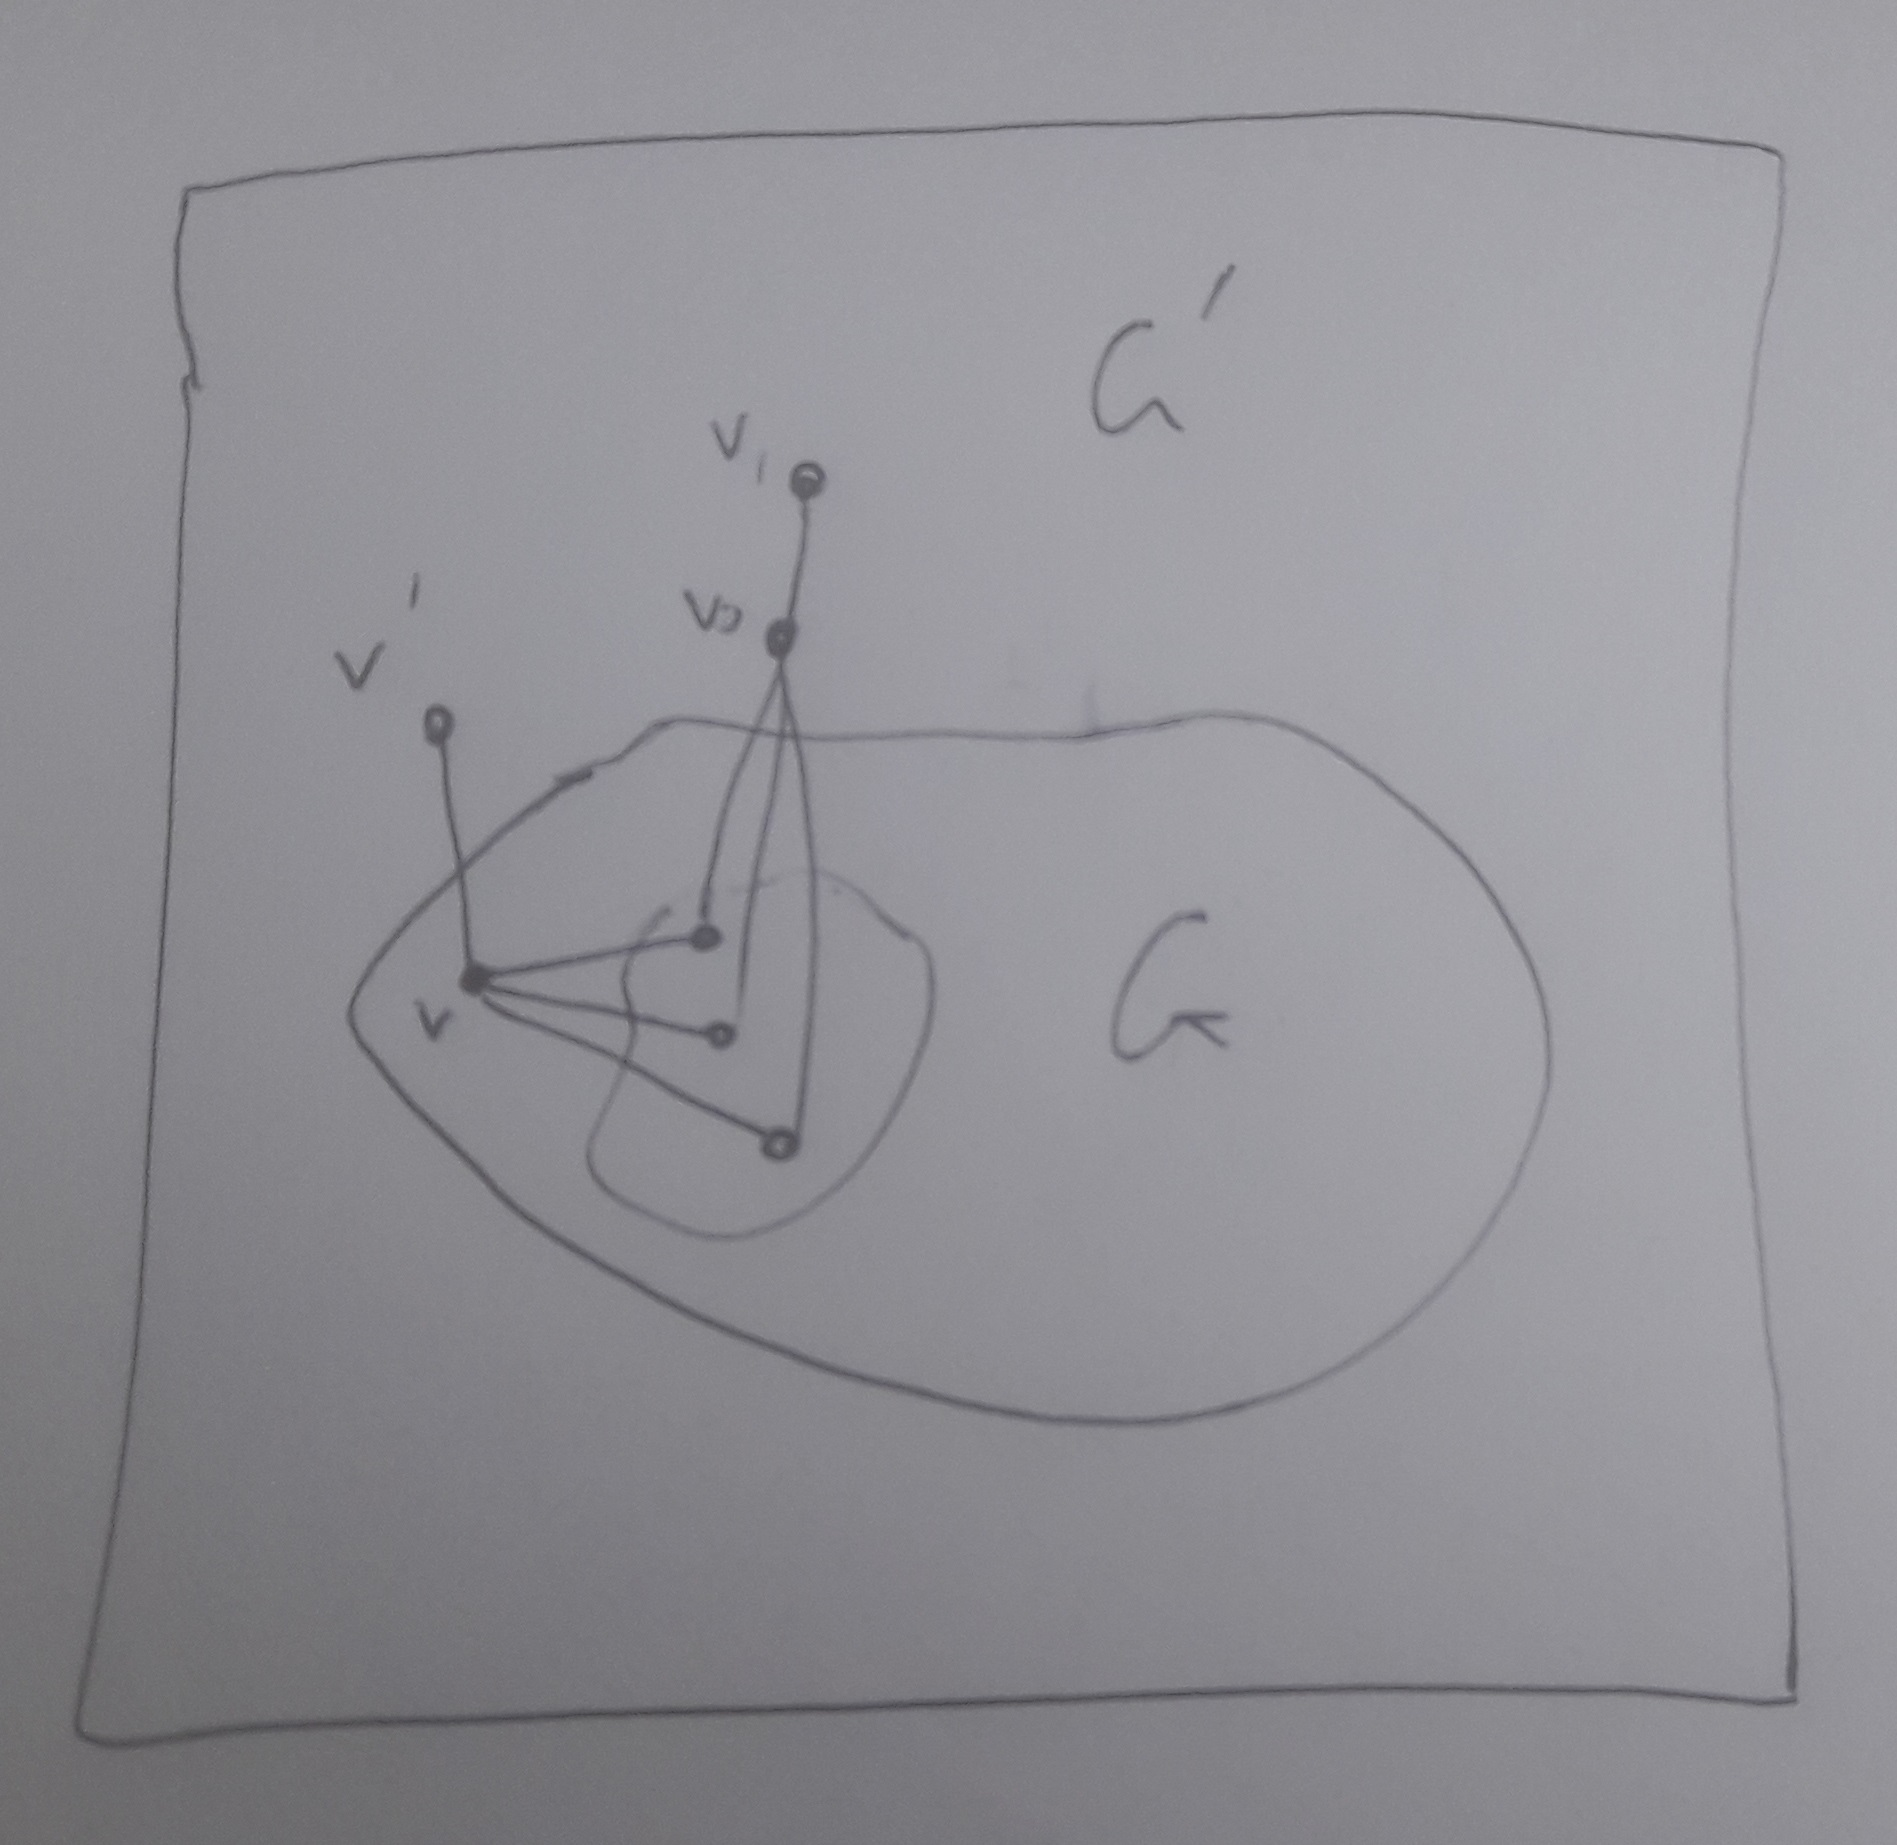
\includegraphics[scale = 0.1]{G.jpg}\]
Assume it takes constant time to choose a vertex $v$, and also that it takes constant time to create vertices. Then constructing the set of vertices of $G'$ is obviously $O(|V|)$. We add one edge to $G'$ for every edge of $G$, two edges $\{v,v'\}$ and $\{v_0,v_1\}$, and then an edge $\{v_0,u\}$ for every edge $\{v,u\}$ of $G$. As usual assuming constant time to create edges, this is $O(|E|) + O(|E|) = O(|E|)$. So the total time is $O(|V|+|E|)$.
Let $u_0,\ldots,u_n$ be a Hamiltonian circuit of $G$, and suppose without loss of generality that $u_0 = v$. Consider the sequence $v',v=u_0,\ldots,u_n,v_0,v_1$ of $G'$. There are obviously no repeated vertices in this sequence. Moreover, there are edges $\{v',v\}$ and $\{v_0,v_1\}$ by construction of $G'$, and, as there is an edge $\{u_n,u_0\}$ in $G$, there is also an edge $\{u_n, v_0\}$. It follows that $v',v,u_0,\ldots,u_n,v_0,v_1$ is a Hamiltonian path.

Conversely, suppose $u_0,u_1,\ldots,u_{m-1},u_m$ is a Hamiltonian path in $G'$. Then we can suppose without loss of generality that $u_0 = v'$, $u_1 = v$, $u_{m-1} = v_0$ and $u_m = v_1$ (as $v'$ and $v_1$ are the only possible endpoints of such a path). It follows that $u_1,\ldots,u_{m-2}$ is a Hamiltonian path in $G$. Moreover, as there is an edge $\{u_{m-2},u_{m-1}\}$ in $G'$ (i.e. from $u_{m-2}$ to $v_0$), there must be an edge $\{u_{m-2},u_1\}$ in $G$ (i.e. from $u_{m-2}$ to $v=u_1$). Thus $u_1,\ldots,u_{m-2}$ is a Hamiltonian circuit as required. 
We have defined a $p$-time reduction as required.

\end{comment}


\end{document}